\section{DODATEK B: Dokumentacja techniczna}
\label{sub:dodatekB}

Projekt został napisany w programie \textit{MATLAB 2017b}. Korzystano z gotowego GUI programu \textit{MATLAB - Neural Network Toolbox} oraz innych funkcji z tego \textit{toolbox}. Baza danych potrzebna do realizacji postawionego zadania została pobrana z źródła.
%link do bazy

\subsection{Dokumentacja oprogramowania}
\label{sub:dokumentacja}

Wszystkie funkcje użyte na potrzeby zaimplementowania algorytmu zostały zaczerpnięte z gotowych rozwiązań. Opis i dokumentacja techniczna GUI \textit{Neural Network Toolbox} znajduje się w źródle \cite{gui}, zaś do funkcji użytych w procesie tworzenia głębokich sieci neuronowych w źródle \cite{funkcje}.

Kolejność użytych funkcji przedstawiono na schemacie \ref{fig:flow}.

\begin{figure}[H]
	\centering
	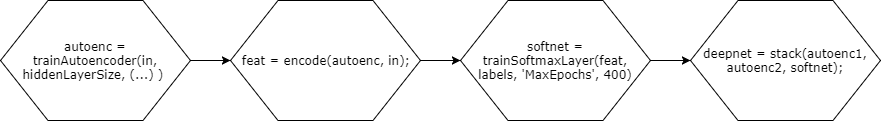
\includegraphics[scale=0.45]{obrazki/flow}
	\caption{\label{fig:subcaption_example}Schemat blokowy użytych funkcji do głębokiego uczenia sieci neuronowej.}{\label{fig:flow}}
\end{figure}

Funkcja \textit{trainAutoencoder} tworzy ukryte warstwy. Jako parametry przyjmuje dane wejściowe, ilość ukrytych warstw oraz parametry określające dynamikę i właściwości wag. Dodatkowo można tu zdecydować, czy obliczenia mają być wykonywane również na procesorze GPU. Funkcja \textit{encode} służy do ekstrakcji cech z ukrytych warstw, a jako parametry przyjmuje dane wejściowe oraz wynik działania autoenkodera. Funkcja \textit{trainSoftmaxLayer} tworzy funkcę aktywacji typu softmax, bazując na cechach zwróconych po wywiłaniu funkcji \textit{encode} oraz etykietach danych wejściowych. Określa się tutaj także maksymalną liczbę epok. Ostatnia funkcja \textit{stack} układa wszystkie warstwy, łącząc stworzone autoenkodery oraz warstwę wyjściową. Funkcja ta tworzy głęboką sieć neuronową, która może być już użyta do testowania.


\subsection{Procedura symulacji, testowania i weryfikacji}
\label{sub:procedura}

Do realizacji projektu nie używano żadnej zewnętrznej platformy sprzętowej. Aby uruchomić aplikację wystarczy komputer PC spełniający wymagania sprzętowo - programowe opisane w sekcji \ref{sub:przygotowanie} z zainstalowanym programem \textit{MATLAB 2017b}. Potrzebny jest także \textit{Neural Network Toolbox}, który będzie wbudowany w przypadku pełnej instalacji programu. W celu przygotowania danych do uczenia można pobrać bazę ze źródła \cite{baza} i uruchomić skrypt \textit{Data$\_$selection} znajdujący się na nośniku CD. Można również wczytać przygotowane już dane w formacie .mat: data$\_$matrix.mat oraz images$\_$double.mat znajdujące się również na nośniku CD. W celu weryfikacji algorytmu należy skorzystać z \textit{Neural Network Toolbox}, wybierając opcję \textit{Pattern recognition and classification}. Jako wejście należy wczytać macierze input$\_$matrix oraz output$\_$matrix. Druga opcja zakłada skorzystanie z głębokiego uczenia z użyciem większej liczby warst ukrytych. W tym celu trzeba uruchomić skrypt \textit{GPU$\_$Mnist} (płyta CD). Należy zaznaczyć, że proces trwa dosyć długo, a liczenie przebiega tu w sposób równoległy i z użyciem procesora graficznego GPU.

